

\begin{frame}{\ft{Viewing Re-PDF Files}}

\doubleFrame{An Re-PDF file serves two purposes: first, 
it embeds pictures and data about 
individual properties so this information can be 
conveniently downloaded and saved, like a zipped folder;  
second, it displays important facts about properties 
--- similar to an MLS website.}

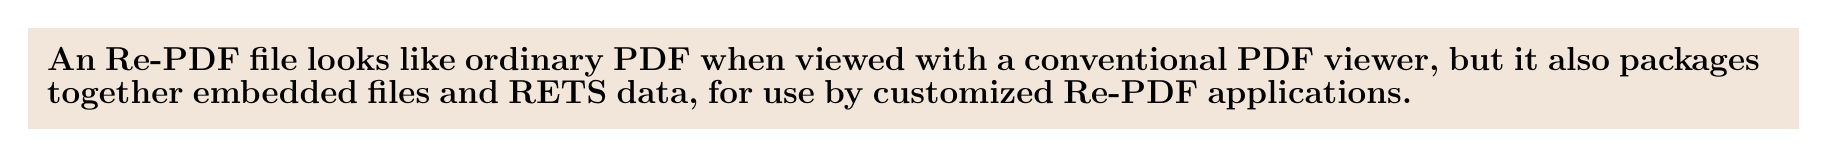
\begin{tikzpicture}
\nodeincludegraphicsTR{6.18cm}{0cm}{screenshots/ss-loaded.png}

 \node [anchor=west,fill=brown!20!white,inner sep=7, text width=22cm]
  (longnote) at (0.5,5) {%  %{\color{rb!85!red}{
  {\cframedbox{\large \textbf{An Re-PDF file looks like 
  ordinary PDF when viewed with a conventional PDF viewer, 
  but it also packages together embedded files 
  and RETS data, for use by customized Re-PDF applications.}}}};


\end{tikzpicture}


\end{frame}

